\section{The Derivative of a Function}
\label{sec:derivative_of_a_function}

\subsection*{Recommended Tutorials:}
\begin{itemize}[noitemsep]
	\item \nameref{chp:assignment_operator}, pg. \pageref{chp:assignment_operator}
	\item \nameref{chp:equation_solvers}, pg. \pageref{chp:equation_solvers}
	\item \nameref{chp:derivative}, pg. \pageref{chp:derivative}
\end{itemize}

\subsection*{Introduction:}

In this activity, we will investigate the derivative of a function and use Maple's powerful computational skills to simplify the process of finding a derivative.

\subsection*{Exercises:}

\begin{enumerate}
    \item  Consider the function $f(x) = \sqrt{9 - x}$.
    \marginnote[-0.2cm]{To input a square root, use the \texttt{sqrt()} command.}  \index{mathematical functions!square root}
    \marginnote[0.2cm]{When assigning the function to $f(x)$, use the $:=$ operator.}
    \begin{enumerate}
    	\item Define this function in Maple.
    	\item Find the derivative\index{derivative}, $f'(x)$, using the \texttt{limit()}\index{limit} command and the limit definition of the derivative.
    	\marginnote[-0.3cm]{Don't forget! \[f'(x) = \dlim{h}{0}\dfrac{f(x+h)-f(x)}{h}\]}\index{limit!definition of a derivative}
    	\item Find the derivative, $f'(x)$, using the \texttt{diff()}\index{derivative!diff} command.
    	\item Find the derivative, $f'(x)$, using \texttt{'}\index{derivative!prime notation} notation.
%    	\item Define the equation of the tangent lines at $x=0$ and $x=5$.
%    	\item Plot $f(x)$ and the two tangent lines on the same axes.
    \end{enumerate}
    \item A toy rocket is fired straight upward, and its height (in metres) is given by: $h(t) = t + 10 - \sqrt{2t^2 + 100}$, with $0 \leq t \leq 20$, where $t$ is the time in seconds.
    \marginnote[-0.8cm]{If you decide to define a height function, be sure that the variable in your function name matches the variable in your function.}
    \begin{enumerate}
    	\item Plot\index{plot} a graph of height as a function of time.
    	\item Find a formula for velocity in terms of $t$.
    	\marginnote[-0.3cm]{Recall that the derivative of position with respect to time is velocity.}
    	\item At what time is the velocity $0$ m/s?
    	\item What is the maximum height that the rocket attains?
    	\marginnote[-0.5cm]{When the velocity of the rocket is $0$ m/s, the rocket has reached its maximum height.}
    	\marginnote[0.5cm]{An example of finding minimum and maximum values on a closed interval can be found on page \pageref{subsec:closed_interval_method}.}
    \end{enumerate}
    \item Molten lava can fill a chamber in the earth's crust before it builds up enough pressure to erupt. Let the pressure be modeled by $P(t) = 0.47 t^2 {\rm e}^{0.0035 t}$, where $t$ is the time in months.
    \marginnote[1cm]{Recall that \texttt{exp()} \index{mathematical functions!exponential} is used to denote the exponential function in Maple.}
    \begin{enumerate}
    	\item What is the rate of change of pressure with respect to time?
    	\item Suppose that an eruption is highly likely to occur if pressure increases at a rate greater than $20$. Is an eruption likely when $t=30$ months? Use a new paragraph to state your answer.
    \end{enumerate}
    \newpage
	\item Consider the function $g(x)=\sin(2\pi^2 x)$.\index{mathematical functions!sine}
		\marginnote[-0.1cm]{To type the mathematical constant $\pi = 3.14\hdots$\index{Pi}, be sure to use \texttt{Pi}. }
		\marginnote[0.1cm]{Don't forget to include multiplication between $\pi^2$ and $x$.}
	\begin{enumerate}
	\item Use Maple to find the first derivative, the second derivative, the third derivative, and the fourth derivative of $g(x)$. You should notice a pattern, so use a new paragraph to describe it.
	\marginnote[-0.1cm]{The $n$\textsuperscript{th} derivative\index{derivative!diff!higher derivatives}\index{derivative!prime notation!higher derivatives} of the function can be computed by using the \texttt{diff()} command or \texttt{'} notation. See page \pageref{chp:derivative} for more information. You can also make use of the Calculus palette:
	\begin{center} 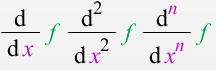
\includegraphics[scale=0.6]{tutorials/figures/palettediff.png}
 \end{center} }
	\item Use your answer from part (a) to predict what the $77$\textsuperscript{th} derivative of $g(x)$ is, and then verify that your prediction is correct by computing this derivative using Maple.
	\item (Optional) Use the information in Tutorial \ref{chp:conditional_statements_and_loops} on page \pageref{chp:conditional_statements_and_loops} to write a loop\index{loops} that will output the first $100$ derivatives of $g(x)$.
	\end{enumerate}
\end{enumerate}

%\subsection*{Notes:}
%\begin{itemize}
%    \item  
%\end{itemize}